% Ce fichier main.tex est le fichier principal \`{a} partir duquel tout est g\'{e}n\'{e}r\'{e}
% This file is the main file where the final document is generated
\documentclass{these-dbl}

% Fill the pdf metadata
\hypersetup{
%    pdfauthor   = {XYZ},
%    pdftitle    = {Th\`{e}se de doctorat de XYZ},
%    pdfsubject  = {Th\`{e}se de doctorat de XYZ},
%    pdfkeywords = {mots-cl\'{e}s},
}

\geometry{vmargin=4.0cm}
\addbibresource{./biblio/biblio.bib}

\makeglossaries
% Acronymes
\newacronym{gcd}{GCD}{Greatest Common Divisor}
\newacronym{lcm}{LCM}{Least Common Multiple}

% Définitions
\newglossaryentry{git}
{%
    name={git},
    description={
    Logiciel de versionnage git, raccourcit pour désigner à la fois un répertoire git ou un projet git sur des plateformes en ligne comme github ou gitlab.
    }
}



\begin{document}

% La page de garde est en français
% The front cover is in French
\selectlanguage{french}

% S8 or S10
\semester{«Semester»}
\entreprise{« Entreprise »}
\author{« Pr\'{e}nom NOM »}
\title{« Titre du stage»}
\date{« date »}
\lieu{« Lieu »}

\jury{
{\normalTwelve \textbf{Composition du Jury :}}\\
\newline
\footnotesizeTwelve
\begin{tabular}{@{}lll}
Tuteur ENIB :          & Pr\'{e}nom NOM & ENIB  \\
Accesseur :          & Pr\'{e}nom NOM & ENIB \\
Tuteur Entreprise :    & Pr\'{e}nom NOM & Fonction et \'{e}tablissement d'exercice \\
\end{tabular}
}

\maketitle



\selectlanguage{french}

\clearemptydoublepage
\chapter*{Remerciements}

Je tiens à remercier  \\
I would like to thank. my parents..\\
J'adresse également toute ma reconnaissance à .... \\
....


\frontmatter
\clearemptydoublepage
\renewcommand{\contentsname}{Table des Matières}
\tableofcontents %sommaire %table of content
%\shorttableofcontents{Sommaire}{0}

\clearemptydoublepage
\listoffigures

\clearemptydoublepage
\listoftables

\clearemptydoublepage
\lstlistoflistings

\clearemptydoublepage
\chapter*{Introduction}
\addcontentsline{toc}{chapter}{Introduction}
\chaptermark{Introduction}


Lorem ipsum dolor sit amet, «~consectetuer~» adipiscing elit. Maecenas fermentum, elit non lobortis cursus, orci velit suscipit est, id mollis turpis mi eget orci. Ut aliquam sollicitudin metus. Mauris at sapien sed sapien congue iaculis. Nulla lorem urna, bibendum id, laoreet iaculis, nonummy eget, massa. Phasellus ullamcorper commodo velit. Class aptent taciti sociosqu ad litora torquent per «~conubia nostra~», per inceptos hymenaeos. Phasellus est. Maecenas felis augue, gravida quis, porta adipiscing, iaculis vitae, felis. Nullam ipsum. Nulla a sem ac leo fringilla mattis. Phasellus egestas augue in sem. Etiam ac enim non mauris ullamcorper scelerisque. In wisi leo, malesuada vulputate, tempor sit amet, facilisis vel, velit. Mauris massa est, sodales placerat, luctus id, hendrerit a, urna. Nullam eleifend pede eget odio. Duis non erat. Nullam pellentesque.

\begin{verse}
Maître Corbeau, sur un arbre perché, \\
Tenait en son bec un fromage. \\
Maître Renard, par l'odeur alléché, \\
Lui tint à peu près ce langage : \\
«~Hé ! bonjour, Monsieur du Corbeau. \\
Que vous êtes joli ! que vous me semblez beau ! \\
Sans mentir, si votre ramage \\
Se rapporte à votre plumage, \\
Vous êtes le Phénix des hôtes de ces bois.~» \\
\end{verse}

Lorem ipsum dolor sit amet, consectetuer adipiscing elit. Maecenas fermentum, elit non lobortis cursus, orci velit suscipit est, id mollis turpis mi eget orci. Ut aliquam sollicitudin metus. Mauris at sapien sed sapien congue iaculis. Nulla lorem urna, bibendum id, laoreet iaculis, nonummy eget, massa\footcite[32]{Pierre1901}. Phasellus ullamcorper commodo velit. Class aptent taciti sociosqu ad litora torquent per conubia nostra, per inceptos hymenaeos. Phasellus est. Maecenas felis augue, gravida quis, porta adipiscing, iaculis vitae, felis. Nullam ipsum. Nulla a sem ac leo fringilla mattis. Phasellus egestas augue in sem. Etiam ac enim non mauris ullamcorper scelerisque. In wisi leo, malesuada vulputate, tempor sit amet, facilisis vel, velit. Mauris massa est, sodales placerat, luctus id, hendrerit a, urna. Nullam eleifend pede eget odio. Duis non erat. Nullam pellentesque. 

\section*{Première section de l'intro}
\addcontentsline{toc}{section}{Première section de l'intro}

Lorem ipsum dolor sit amet, «~consectetuer~» adipiscing elit. Maecenas fermentum, elit non lobortis cursus, orci velit suscipit est, id mollis turpis mi eget orci. Ut aliquam sollicitudin metus. Mauris at sapien sed sapien congue iaculis. Nulla lorem urna, bibendum id, laoreet iaculis, nonummy eget, massa. Phasellus ullamcorper commodo velit. Class aptent taciti sociosqu ad litora torquent per «~conubia nostra~», per inceptos hymenaeos. Phasellus est. Maecenas felis augue, gravida quis, porta adipiscing, iaculis vitae, felis. Nullam ipsum. Nulla a sem ac leo fringilla mattis. Phasellus egestas augue in sem. Etiam ac enim non mauris ullamcorper scelerisque. In wisi leo, malesuada vulputate, tempor sit amet, facilisis vel, velit. Mauris massa est, sodales placerat, luctus id, hendrerit a, urna. Nullam eleifend pede eget odio. Duis non erat. Nullam pellentesque.

\textbf{Une boite magique : }

\boitemagique{Titre de la boite}{
Praesent placerat, ante at venenatis pretium, diam turpis faucibus arcu, nec vehicula quam lorem ut leo. Sed facilisis, augue in pharetra dapibus, ligula justo accumsan massa, eu suscipit felis ipsum eget enim.
}

Laoreet iaculis, nonummy eget, massa. Phasellus ullamcorper commodo velit. Class aptent taciti sociosqu ad litora torquent per «~conubia nostra~», per inceptos hymenaeos. Phasellus est. Maecenas felis augue, gravida quis, porta adipiscing, iaculis vitae, felis. Nullam ipsum. Nulla a sem ac leo fringilla mattis. Phasellus egestas augue in sem. Etiam ac enim non mauris ullamcorper scelerisque. In wisi leo, malesuada vulputate, tempor sit amet, facilisis vel, velit. Mauris massa est, sodales placerat, luctus id, hendrerit a, urna. Nullam eleifend pede eget odio. Duis non erat. Nullam pellentesque.

\textbf{Une boite simple : }
\boitesimple{Mauris lorem quam, tristique sollicitudin egestas sed, sodales vel leo. In hac habitasse platea dictumst. Lorem ipsum dolor sit amet, consectetur adipiscing elit. Sed sed lorem lacus, at venenatis elit. Pellentesque nisl arcu, blandit ac eleifend non, sodales a quam.}

Laoreet iaculis, nonummy eget, massa. Phasellus ullamcorper commodo velit. Class aptent taciti sociosqu ad litora torquent per «~conubia nostra~», per inceptos hymenaeos. Phasellus est. Maecenas felis augue, gravida quis, porta adipiscing, iaculis vitae, felis. Nullam ipsum. Nulla a sem ac leo fringilla mattis. Phasellus egestas augue in sem. Etiam ac enim non mauris ullamcorper scelerisque. In wisi leo, malesuada vulputate, tempor sit amet, facilisis vel, velit. Mauris massa est, sodales placerat, luctus id, hendrerit a, urna. Nullam eleifend pede eget odio. Duis non erat. Nullam pellentesque.




\clearemptydoublepage
\mainmatter
\clearemptydoublepage
\chapter{Présentation du Stage}


Morbi lorem. Etiam scelerisque rhoncus orci. Nunc elementum ante ac leo. Vestibulum venenatis dictum nunc. Donec turpis est, dictum nec, fringilla nec, cursus id, quam. In nibh orci, porttitor ut, rutrum id, faucibus vitae, leo. Donec ut wisi. Vivamus ornare, lorem quis tristique dapibus, nulla nisl nonummy libero, vitae luctus sem felis vel nisl. Suspendisse lectus lacus, ultricies vitae, feugiat et, hendrerit in, quam. Pellentesque porttitor enim at lectus. Praesent viverra laoreet velit. Mauris neque odio, ornare id, rhoncus non, sollicitudin sed, lectus. Phasellus et dolor. Aenean ullamcorper risus id libero. Pellentesque ac sem eget libero aliquam tincidunt. Suspendisse neque. Curabitur egestas neque ultrices nisl. Nulla bibendum augue et tellus. Duis ultrices convallis est.


\clearemptydoublepage
\clearemptydoublepage
\chapter{Titre du second chapitre}

Lorem ipsum dolor sit amet, «~consectetuer~» adipiscing elit. Maecenas fermentum, elit non lobortis cursus, orci velit suscipit est, id mollis turpis mi eget orci. Ut aliquam sollicitudin metus. Mauris at sapien sed sapien congue iaculis. Nulla lorem urna, bibendum id, laoreet iaculis, nonummy eget, massa. Phasellus ullamcorper commodo velit. Class aptent taciti sociosqu ad litora torquent per «~conubia nostra~», per inceptos hymenaeos. Phasellus est. Maecenas felis augue, gravida quis, porta adipiscing, iaculis vitae, felis. Nullam ipsum. Nulla a sem ac leo fringilla mattis. Phasellus egestas augue in sem. Etiam ac enim non mauris ullamcorper scelerisque. In wisi leo, malesuada vulputate, tempor sit amet, facilisis vel, velit. Mauris massa est, sodales placerat, luctus id, hendrerit a, urna. Nullam eleifend pede eget odio. Duis non erat. Nullam pellentesque.

Lorem ipsum dolor sit amet, consectetuer adipiscing elit. Maecenas fermentum, elit non lobortis cursus, orci velit suscipit est, id mollis turpis mi eget orci. Ut aliquam sollicitudin metus. Mauris at sapien sed sapien congue iaculis. Nulla lorem urna, bibendum id, laoreet iaculis, nonummy eget, massa\footcite[12]{Pierre1901}. Phasellus ullamcorper commodo velit. Class aptent taciti sociosqu ad litora torquent per conubia nostra, per inceptos hymenaeos. Phasellus est. Maecenas felis augue, gravida quis, porta adipiscing, iaculis vitae, felis. Nullam ipsum. Nulla a sem ac leo fringilla mattis. Phasellus egestas augue in sem. Etiam ac enim non mauris ullamcorper scelerisque. In wisi leo, malesuada vulputate, tempor sit amet, facilisis vel, velit. Mauris massa est, sodales placerat, luctus id, hendrerit a, urna. Nullam eleifend pede eget odio. Duis non erat. Nullam pellentesque. 

\section{Première section du chapitre}

\subsection{Première sous-section}

Cras molestie. Curabitur id urna. Suspendisse tempor. Aliquam erat volutpat. Aliquam erat volutpat. Nam ultricies metus sit amet erat\footnote{Mauris neque odio, ornare id, rhoncus non, sollicitudin sed, lectus. Phasellus et dolor. Aenean ullamcorper risus id libero. Pellentesque ac sem eget libero aliquam tincidunt. Suspendisse neque.}. Suspendisse eget ipsum ut purus imperdiet suscipit. Mauris sed urna at diam volutpat placerat. Nulla vitae tortor. Nulla sed nisl.

Lorem ipsum dolor sit amet, consectetuer adipiscing elit. Maecenas fermentum, elit non lobortis cursus, orci velit suscipit est, id mollis turpis mi eget orci. Ut aliquam sollicitudin metus. Mauris at sapien sed sapien congue iaculis. Nulla lorem urna, bibendum id, laoreet iaculis, nonummy eget, massa. Phasellus ullamcorper commodo velit. Class aptent taciti sociosqu ad litora torquent per conubia nostra, per inceptos hymenaeos. Phasellus est. Maecenas felis augue, gravida quis, porta adipiscing, iaculis vitae, felis. Nullam ipsum. Nulla a sem ac leo fringilla mattis. Phasellus egestas augue in sem. Etiam ac enim non mauris ullamcorper scelerisque. In wisi leo, malesuada vulputate, tempor sit amet, facilisis vel, velit. Mauris massa est, sodales placerat, luctus id, hendrerit a, urna. Nullam eleifend pede eget odio. Duis non erat. Nullam pellentesque\footcite[56]{Desfois1998}.


\begin{quote}
Aenean ullamcorper risus id libero. Pellentesque ac sem eget libero aliquam tincidunt. Suspendisse neque. Rutrum id, faucibus vitae, leo. Donec ut wisi. Vivamus ornare, lorem quis tristique dapibus, nulla nisl nonummy libero, vitae luctus sem felis vel nisl. Suspendisse lectus lacus, ultricies vitae, feugiat et, hendrerit in, quam. Pellentesque porttitor enim at lectus. Praesent viverra laoreet velit. Mauris neque odio, ornare id, rhoncus non, sollicitudin sed, lectus. Aenean ullamcorper risus id libero. Pellentesque ac sem eget libero aliquam tincidunt. Suspendisse neque\footcite[voir \pno~154]{Georges1974}.
\end{quote}

Morbi lorem. Etiam scelerisque rhoncus orci\footcite{Georges1974}. Nunc elementum ante ac leo. Vestibulum venenatis dictum nunc. Donec turpis est, dictum nec, fringilla nec, cursus id, quam. In nibh orci, porttitor ut, rutrum id, faucibus vitae, leo. Donec ut wisi. Vivamus ornare, lorem quis tristique dapibus, nulla nisl nonummy libero, vitae luctus sem felis vel nisl. Suspendisse lectus lacus, ultricies vitae, feugiat et, hendrerit in, quam. Pellentesque porttitor enim at lectus. Praesent viverra laoreet velit\footcite[56]{Desfois1998}. Mauris neque odio, ornare id, rhoncus non, sollicitudin sed, lectus. Phasellus et dolor. Aenean ullamcorper risus id libero. Pellentesque ac sem eget libero aliquam tincidunt. Suspendisse neque. Curabitur egestas neque ultrices nisl. Nulla bibendum augue et tellus. Duis ultrices convallis est.

Lorem ipsum dolor sit amet, consectetuer adipiscing elit. Maecenas fermentum, elit non lobortis cursus, orci velit suscipit est, id mollis turpis mi eget orci. Ut aliquam sollicitudin metus. Mauris at sapien sed sapien congue iaculis. Nulla lorem urna, bibendum id, laoreet iaculis, nonummy eget, massa. Phasellus ullamcorper commodo velit. Class aptent taciti sociosqu ad litora torquent per conubia nostra, per inceptos hymenaeos. Phasellus est. Maecenas felis augue, gravida quis, porta adipiscing, iaculis vitae, felis. Nullam ipsum. Nulla a sem ac leo fringilla mattis. Phasellus egestas augue in sem. Etiam ac enim non mauris ullamcorper scelerisque. In wisi leo, malesuada vulputate, tempor sit amet, facilisis vel, velit. Mauris massa est, sodales placerat, luctus id, hendrerit a, urna. Nullam eleifend pede eget odio. Duis non erat. Nullam pellentesque.

Lorem ipsum dolor sit amet, consectetuer adipiscing elit. Maecenas fermentum, elit non lobortis cursus, orci velit suscipit est, id mollis turpis mi eget orci. Ut aliquam sollicitudin metus. Mauris at sapien sed sapien congue iaculis. Nulla lorem urna, bibendum id, laoreet iaculis, nonummy eget, massa. Phasellus ullamcorper commodo velit. Class aptent taciti sociosqu ad litora torquent per conubia nostra, per inceptos hymenaeos. Phasellus est. Maecenas felis augue, gravida quis, porta adipiscing, iaculis vitae, felis. Nullam ipsum. Nulla a sem ac leo fringilla mattis. Phasellus egestas augue in sem. Etiam ac enim non mauris ullamcorper scelerisque. In wisi leo, malesuada vulputate, tempor sit amet, facilisis vel, velit. Mauris massa est, sodales placerat, luctus id, hendrerit a, urna. Nullam eleifend pede eget odio. Duis non erat. Nullam pellentesque.
Voir figure \ref{fig:mafigure2}.

\begin{figure}[ht]
   \begin{center}
      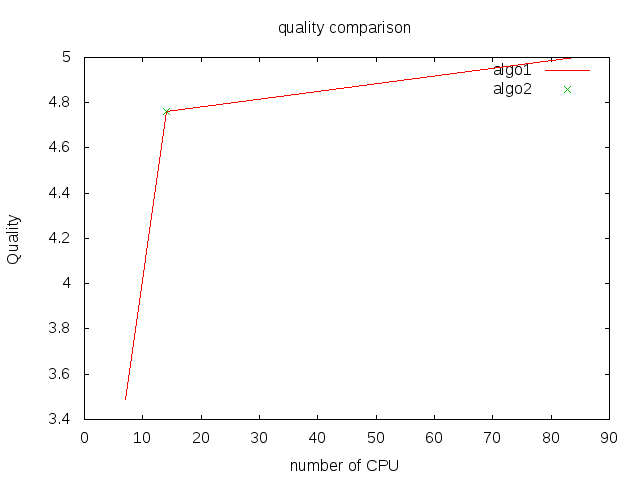
\includegraphics[width=0.6\linewidth]{chapter2/figures/comparison.png}
   \end{center}
   \caption[titre court pour la liste des figures]
   {\footnotesize Titre plus long avec des explications.}
   \label{fig:mafigure2}
\end{figure}


\subsection{Deuxième sous-section}

Morbi lorem. Etiam scelerisque rhoncus orci. Nunc elementum ante ac leo. Vestibulum venenatis dictum nunc. Donec turpis est, dictum nec, fringilla nec, cursus id, quam. In nibh orci, porttitor ut, rutrum id, faucibus vitae, leo. Donec ut wisi. Vivamus ornare, lorem quis tristique dapibus, nulla nisl nonummy libero, vitae luctus sem felis vel nisl. Suspendisse lectus lacus, ultricies vitae, feugiat et, hendrerit in, quam. Pellentesque porttitor enim at lectus. Praesent viverra laoreet velit. Mauris neque odio, ornare id, rhoncus non, sollicitudin sed, lectus. Phasellus et dolor. Aenean ullamcorper risus id libero. Pellentesque ac sem eget libero aliquam tincidunt. Suspendisse neque. Curabitur egestas neque ultrices nisl. Nulla bibendum augue et tellus. Duis ultrices convallis est.

Lorem ipsum dolor sit amet, consectetuer adipiscing elit. Maecenas fermentum, elit non lobortis cursus, orci velit suscipit est, id mollis turpis mi eget orci. Ut aliquam sollicitudin metus. Mauris at sapien sed sapien congue iaculis. Nulla lorem urna, bibendum id, laoreet iaculis, nonummy eget, massa. Phasellus ullamcorper commodo velit. Class aptent taciti sociosqu ad litora torquent per conubia nostra, per inceptos hymenaeos. Phasellus est. Maecenas felis augue, gravida quis, porta adipiscing, iaculis vitae, felis. Nullam ipsum. Nulla a sem ac leo fringilla mattis. Phasellus egestas augue in sem. Etiam ac enim non mauris ullamcorper scelerisque. In wisi leo, malesuada vulputate, tempor sit amet, facilisis vel, velit. Mauris massa est, sodales placerat, luctus id, hendrerit a, urna. Nullam eleifend pede eget odio. Duis non erat. Nullam pellentesque.

Lorem ipsum dolor sit amet, consectetuer adipiscing elit. Maecenas fermentum, elit non lobortis cursus, orci velit suscipit est, id mollis turpis mi eget orci. Ut aliquam sollicitudin metus. Mauris at sapien sed sapien congue iaculis. Nulla lorem urna, bibendum id, laoreet iaculis, nonummy eget, massa. Phasellus ullamcorper commodo velit. Class aptent taciti sociosqu ad litora torquent per conubia nostra, per inceptos hymenaeos. Phasellus est. Maecenas felis augue, gravida quis, porta adipiscing, iaculis vitae, felis. Nullam ipsum. Nulla a sem ac leo fringilla mattis. Phasellus egestas augue in sem. Etiam ac enim non mauris ullamcorper scelerisque. In wisi leo, malesuada vulputate, tempor sit amet, facilisis vel, velit. Mauris massa est, sodales placerat, luctus id, hendrerit a, urna. Nullam eleifend pede eget odio. Duis non erat. Nullam pellentesque.

Lorem ipsum dolor sit amet, consectetuer adipiscing elit. Maecenas fermentum, elit non lobortis cursus, orci velit suscipit est, id mollis turpis mi eget orci. Ut aliquam sollicitudin metus. Mauris at sapien sed sapien congue iaculis. Nulla lorem urna, bibendum id, laoreet iaculis, nonummy eget, massa. Phasellus ullamcorper commodo velit. Class aptent taciti sociosqu ad litora torquent per conubia nostra, per inceptos hymenaeos. Phasellus est. Maecenas felis augue, gravida quis, porta adipiscing, iaculis vitae, felis. Nullam ipsum. Nulla a sem ac leo fringilla mattis. Phasellus egestas augue in sem. Etiam ac enim non mauris ullamcorper scelerisque. In wisi leo, malesuada vulputate, tempor sit amet, facilisis vel, velit. Mauris massa est, sodales placerat, luctus id, hendrerit a, urna. Nullam eleifend pede eget odio. Duis non erat. Nullam pellentesque.

\section{Affichage de courbes}

\subsubsection{Modélisation Mathématique}

Une sinusoide peut être modélisée mathématiquement par :
\begin{align}
x(t) = \sin(2\pi f_0 t)
\end{align}

La figure \ref{fig:mafigure3} présente l'allure d'une sinusoide avec $f_0=5$Hz.

\begin{figure}[h]
   \begin{center}
      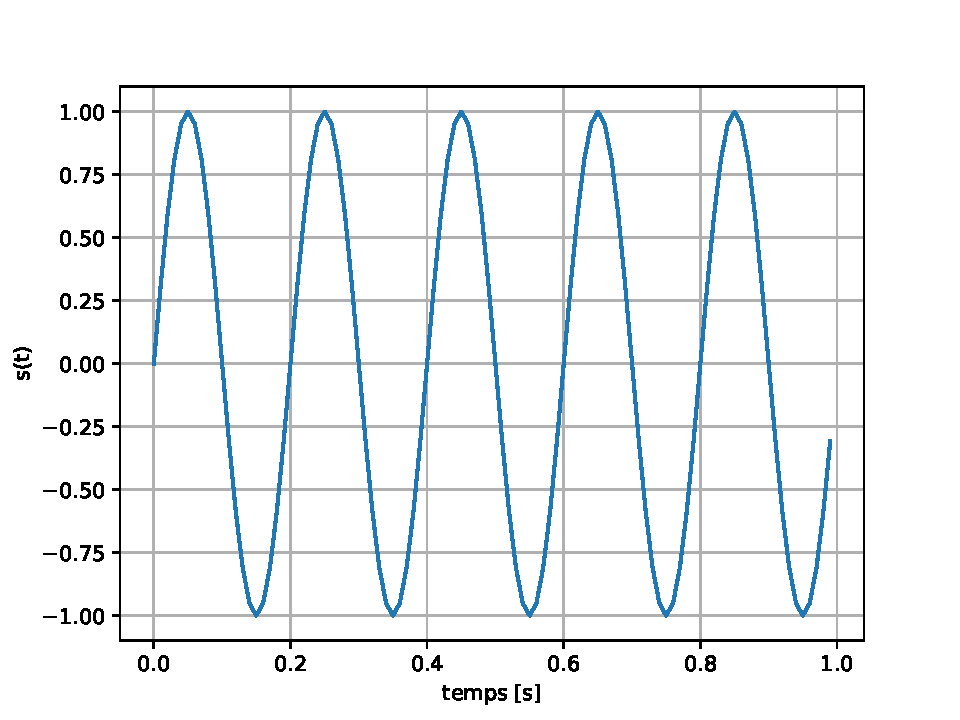
\includegraphics[width=0.6\linewidth]{chapter2/figures/sinewave.pdf}
   \end{center}
   \caption{Sinusoide de fréquence $f_0=5$Hz.}
   \label{fig:mafigure3}
\end{figure}

Lorem ipsum dolor sit amet, consectetuer adipiscing elit. Maecenas fermentum, elit non lobortis cursus, orci velit suscipit est, id mollis turpis mi eget orci. Ut aliquam sollicitudin metus. Mauris at sapien sed sapien congue iaculis. Nulla lorem urna, bibendum id, laoreet iaculis, nonummy eget, massa. Phasellus ullamcorper commodo velit. Class aptent taciti sociosqu ad litora torquent per conubia nostra, per inceptos hymenaeos. Phasellus est. Maecenas felis augue, gravida quis, porta adipiscing, iaculis vitae, felis. Nullam ipsum. Nulla a sem ac leo fringilla mattis. Phasellus egestas augue in sem. Etiam ac enim non mauris ullamcorper scelerisque. In wisi leo, malesuada vulputate, tempor sit amet, facilisis vel, velit. Mauris massa est, sodales placerat, luctus id, hendrerit a, urna. Nullam eleifend pede eget odio. Duis non erat. Nullam pellentesque.


\section{Affichage de tableaux}

La table \ref{table:matable1} présente un tableau latex.


\begin{table}[!h]
   \begin{center}
   \begin{tabular}{||c c c c||} 
    \hline
    Col1 & Col2 & Col2 & Col3 \\ [0.5ex] 
    \hline\hline
    1 & 6 & 87837 & 787 \\ 
    \hline
    2 & 7 & 78 & 5415 \\
    \hline
    3 & 545 & 778 & 7507 \\
    \hline
    4 & 545 & 18744 & 7560 \\
    \hline
    5 & 88 & 788 & 6344 \\ [1ex] 
    \hline
   \end{tabular}
   \end{center}
   \caption{Un titre pour mes données.}
   \label{table:matable1}
\end{table}

Morbi lorem. Etiam scelerisque rhoncus orci. Nunc elementum ante ac leo. Vestibulum venenatis dictum nunc. Donec turpis est, dictum nec, fringilla nec, cursus id, quam. In nibh orci, porttitor ut, rutrum id, faucibus vitae, leo. Donec ut wisi. Vivamus ornare, lorem quis tristique dapibus, nulla nisl nonummy libero, vitae luctus sem felis vel nisl. Suspendisse lectus lacus, ultricies vitae, feugiat et, hendrerit in, quam. Pellentesque porttitor enim at lectus. Praesent viverra laoreet velit. Mauris neque odio, ornare id, rhoncus non, sollicitudin sed, lectus. Phasellus et dolor. Aenean ullamcorper risus id libero. Pellentesque ac sem eget libero aliquam tincidunt. Suspendisse neque. Curabitur egestas neque ultrices nisl. Nulla bibendum augue et tellus. Duis ultrices convallis est.

\section{Affichage de code}

\lstinputlisting[frame=single,language=Python, caption=Exemple Python,captionpos=b]{chapter2/src/sinewave.py}

Morbi lorem. Etiam scelerisque rhoncus orci. Nunc elementum ante ac leo. Vestibulum venenatis dictum nunc. Donec turpis est, dictum nec, fringilla nec, cursus id, quam. In nibh orci, porttitor ut, rutrum id, faucibus vitae, leo. Donec ut wisi. Vivamus ornare, lorem quis tristique dapibus, nulla nisl nonummy libero, vitae luctus sem felis vel nisl. Suspendisse lectus lacus, ultricies vitae, feugiat et, hendrerit in, quam. Pellentesque porttitor enim at lectus. Praesent viverra laoreet velit. Mauris neque odio, ornare id, rhoncus non, sollicitudin sed, lectus. Phasellus et dolor. Aenean ullamcorper risus id libero. Pellentesque ac sem eget libero aliquam tincidunt. Suspendisse neque. Curabitur egestas neque ultrices nisl. Nulla bibendum augue et tellus. Duis ultrices convallis est.


\section{Gestion des Acronymes}

La définiton des acronymes se trouve dans le fichier \texttt{glossary.tex}. Il est possible 
d'obtenir des acronymes longs comme \acrlong{gcd} et des acronymes cours comme \acrshort{gcd}. \\
L'ont peut également définir des termes: \gls{git}.



\clearemptydoublepage
\mainmatter
\chapter[Ceci est un long titre]{Nom du chapitre 2}

Lorem ipsum dolor sit amet, «~consectetuer~» adipiscing elit. Maecenas fermentum, elit non lobortis cursus, orci velit suscipit est, id mollis turpis mi eget orci. Ut aliquam sollicitudin metus. Mauris at sapien sed sapien congue iaculis. Nulla lorem urna, bibendum id, laoreet iaculis, nonummy eget, massa. Phasellus ullamcorper commodo velit. Class aptent taciti sociosqu ad litora torquent per «~conubia nostra~», per inceptos hymenaeos. Phasellus est. Maecenas felis augue, gravida quis, porta adipiscing, iaculis vitae, felis. Nullam ipsum. Nulla a sem ac leo fringilla mattis. Phasellus egestas augue in sem. Etiam ac enim non mauris ullamcorper scelerisque. In wisi leo, malesuada vulputate, tempor sit amet, facilisis vel, velit. Mauris massa est, sodales placerat, luctus id, hendrerit a, urna. Nullam eleifend pede eget odio. Duis non erat. Nullam pellentesque\footcite[225]{Doule1887}.

\section{Première section du chapitre}

\subsection{Première sous-section}

Cras molestie. Curabitur id urna. Suspendisse tempor. Aliquam erat volutpat. Aliquam erat volutpat. Nam ultricies metus sit amet erat\footnote{Mauris neque odio, ornare id, rhoncus non, sollicitudin sed, lectus. Phasellus et dolor. Aenean ullamcorper risus id libero. Pellentesque ac sem eget libero aliquam tincidunt. Suspendisse neque.}. Suspendisse eget ipsum ut purus imperdiet suscipit. Mauris sed urna at diam volutpat placerat. Nulla vitae tortor. Nulla sed nisl.

Morbi lorem. Etiam scelerisque rhoncus orci. Nunc elementum ante ac leo. Vestibulum venenatis dictum nunc. Donec turpis est, dictum nec\footcite[228]{Drocher2006}, fringilla nec, cursus id, quam. In nibh orci, porttitor ut, rutrum id, faucibus vitae, leo. Donec ut wisi. Vivamus ornare, lorem quis tristique dapibus, nulla nisl nonummy libero, vitae luctus sem felis vel nisl. Suspendisse lectus lacus, ultricies vitae, feugiat et, hendrerit in, quam. Pellentesque porttitor enim at lectus. Praesent viverra laoreet velit. Mauris neque odio, ornare id, rhoncus non, sollicitudin sed, lectus. Phasellus et dolor. Aenean ullamcorper risus id libero. Pellentesque ac sem eget libero aliquam tincidunt. Suspendisse neque. Curabitur egestas neque ultrices nisl. Nulla bibendum augue et tellus. Duis ultrices convallis est.

Lorem ipsum dolor sit amet, consectetuer adipiscing elit. Maecenas fermentum, elit non lobortis cursus, orci velit suscipit est, id mollis turpis mi eget orci. Ut aliquam sollicitudin metus. Mauris at sapien sed sapien congue iaculis. Nulla lorem urna, bibendum id, laoreet iaculis, nonummy eget, massa. Phasellus ullamcorper commodo velit. Class aptent taciti sociosqu ad litora torquent per conubia nostra, per inceptos hymenaeos. Phasellus est. Maecenas felis augue, gravida quis, porta adipiscing, iaculis vitae, felis. Nullam ipsum. Nulla a sem ac leo fringilla mattis. Phasellus egestas augue in sem. Etiam ac enim non mauris ullamcorper scelerisque. In wisi leo, malesuada vulputate, tempor sit amet, facilisis vel, velit. Mauris massa est, sodales placerat, luctus id, hendrerit a, urna. Nullam eleifend pede eget odio. Duis non erat. Nullam pellentesque.


\subsection{Deuxième sous-section}

Morbi lorem. Etiam scelerisque rhoncus orci. Nunc elementum ante ac leo. Vestibulum venenatis dictum nunc. Donec turpis est, dictum nec, fringilla nec, cursus id, quam. In nibh orci, porttitor ut, rutrum id, faucibus vitae, leo. Donec ut wisi. Vivamus ornare, lorem quis tristique dapibus, nulla nisl nonummy libero, vitae luctus sem felis vel nisl. Suspendisse lectus lacus, ultricies vitae, feugiat et, hendrerit in, quam. Pellentesque porttitor enim at lectus. Praesent viverra laoreet velit. Mauris neque odio, ornare id, rhoncus non, sollicitudin sed, lectus. Phasellus et dolor. Aenean ullamcorper risus id libero. Pellentesque ac sem eget libero aliquam tincidunt. Suspendisse neque. Curabitur egestas neque ultrices nisl. Nulla bibendum augue et tellus. Duis ultrices convallis est.

Lorem ipsum dolor sit amet, consectetuer adipiscing elit. Maecenas fermentum, elit non lobortis cursus, orci velit suscipit est, id mollis turpis mi eget orci. Ut aliquam sollicitudin metus. Mauris at sapien sed sapien congue iaculis. Nulla lorem urna, bibendum id, laoreet iaculis, nonummy eget, massa. Phasellus ullamcorper commodo velit. Class aptent taciti sociosqu ad litora torquent per conubia nostra, per inceptos hymenaeos. Phasellus est. Maecenas felis augue, gravida quis, porta adipiscing, iaculis vitae, felis. Nullam ipsum. Nulla a sem ac leo fringilla mattis. Phasellus egestas augue in sem. Etiam ac enim non mauris ullamcorper scelerisque. In wisi leo, malesuada vulputate, tempor sit amet, facilisis vel, velit. Mauris massa est, sodales placerat, luctus id, hendrerit a, urna. Nullam eleifend pede eget odio. Duis non erat. Nullam pellentesque.

Lorem ipsum dolor sit amet, consectetuer adipiscing elit. Maecenas fermentum, elit non lobortis cursus, orci velit suscipit est, id mollis turpis mi eget orci. Ut aliquam sollicitudin metus. Mauris at sapien sed sapien congue iaculis. Nulla lorem urna, bibendum id, laoreet iaculis, nonummy eget, massa. Phasellus ullamcorper commodo velit. Class aptent taciti sociosqu ad litora torquent per conubia nostra, per inceptos hymenaeos. Phasellus est. Maecenas felis augue, gravida quis, porta adipiscing, iaculis vitae, felis. Nullam ipsum. Nulla a sem ac leo fringilla mattis. Phasellus egestas augue in sem. Etiam ac enim non mauris ullamcorper scelerisque. In wisi leo, malesuada vulputate, tempor sit amet, facilisis vel, velit. Mauris massa est, sodales placerat, luctus id, hendrerit a, urna. Nullam eleifend pede eget odio. Duis non erat. Nullam pellentesque.

\section{Conclusion}


Lorem ipsum dolor sit amet, consectetuer adipiscing elit. Maecenas fermentum, elit non lobortis cursus, orci velit suscipit est, id mollis turpis mi eget orci. Ut aliquam sollicitudin metus. Mauris at sapien sed sapien congue iaculis. Nulla lorem urna, bibendum id, laoreet iaculis, nonummy eget, massa. Phasellus ullamcorper commodo velit. Class aptent taciti sociosqu ad litora torquent per conubia nostra, per inceptos hymenaeos. Phasellus est. Maecenas felis augue, gravida quis, porta adipiscing, iaculis vitae, felis. Nullam ipsum. Nulla a sem ac leo fringilla mattis. Phasellus egestas augue in sem. Etiam ac enim non mauris ullamcorper scelerisque. In wisi leo, malesuada vulputate, tempor sit amet, facilisis vel, velit. Mauris massa est, sodales placerat, luctus id, hendrerit a, urna. Nullam eleifend pede eget odio. Duis non erat. Nullam pellentesque.

Lorem ipsum dolor sit amet, consectetuer adipiscing elit. Maecenas fermentum, elit non lobortis cursus, orci velit suscipit est, id mollis turpis mi eget orci. Ut aliquam sollicitudin metus. Mauris at sapien sed sapien congue iaculis. Nulla lorem urna, bibendum id, laoreet iaculis, nonummy eget, massa. Phasellus ullamcorper commodo velit. Class aptent taciti sociosqu ad litora torquent per conubia nostra, per inceptos hymenaeos. Phasellus est. Maecenas felis augue, gravida quis, porta adipiscing, iaculis vitae, felis. Nullam ipsum. Nulla a sem ac leo fringilla mattis. Phasellus egestas augue in sem. Etiam ac enim non mauris ullamcorper scelerisque. In wisi leo, malesuada vulputate, tempor sit amet, facilisis vel, velit. Mauris massa est, sodales placerat, luctus id, hendrerit a, urna. Nullam eleifend pede eget odio. Duis non erat. Nullam pellentesque.


\clearemptydoublepage
\backmatter
\chapter*{Conclusion}
\addcontentsline{toc}{chapter}{Conclusion}
\chaptermark{Conclusion}


Lorem ipsum dolor sit amet, «~consectetuer~» adipiscing elit. Maecenas fermentum, elit non lobortis cursus, orci velit suscipit est, id mollis turpis mi eget orci. Ut aliquam sollicitudin metus. Mauris at sapien sed sapien congue iaculis. Nulla lorem urna, bibendum id, laoreet iaculis, nonummy eget, massa. Phasellus ullamcorper commodo velit. Class aptent taciti sociosqu ad litora torquent per «~conubia nostra~», per inceptos hymenaeos. Phasellus est. Maecenas felis augue, gravida quis, porta adipiscing, iaculis vitae, felis. Nullam ipsum. Nulla a sem ac leo fringilla mattis. Phasellus egestas augue in sem. Etiam ac enim non mauris ullamcorper scelerisque. In wisi leo, malesuada vulputate, tempor sit amet, facilisis vel, velit. Mauris massa est, sodales placerat, luctus id, hendrerit a, urna. Nullam eleifend pede eget odio. Duis non erat. Nullam pellentesque.

\begin{verse}
Maître Corbeau, sur un arbre perché, \\
Tenait en son bec un fromage. \\
Maître Renard, par l'odeur alléché, \\
Lui tint à peu près ce langage : \\
«~Hé ! bonjour, Monsieur du Corbeau. \\
Que vous êtes joli ! que vous me semblez beau ! \\
Sans mentir, si votre ramage \\
Se rapporte à votre plumage, \\
Vous êtes le Phénix des hôtes de ces bois.~» \\
\end{verse}

Lorem ipsum dolor sit amet, consectetuer adipiscing elit. Maecenas fermentum, elit non lobortis cursus, orci velit suscipit est, id mollis turpis mi eget orci. Ut aliquam sollicitudin metus. Mauris at sapien sed sapien congue iaculis. Nulla lorem urna, bibendum id, laoreet iaculis, nonummy eget, massa\footcite[32]{Pierre1901}. Phasellus ullamcorper commodo velit. Class aptent taciti sociosqu ad litora torquent per conubia nostra, per inceptos hymenaeos. Phasellus est. Maecenas felis augue, gravida quis, porta adipiscing, iaculis vitae, felis. Nullam ipsum. Nulla a sem ac leo fringilla mattis. Phasellus egestas augue in sem. Etiam ac enim non mauris ullamcorper scelerisque. In wisi leo, malesuada vulputate, tempor sit amet, facilisis vel, velit. Mauris massa est, sodales placerat, luctus id, hendrerit a, urna. Nullam eleifend pede eget odio. Duis non erat. Nullam pellentesque. 

\section*{Première section de l'intro}
\addcontentsline{toc}{section}{Première section de l'intro}

Lorem ipsum dolor sit amet, «~consectetuer~» adipiscing elit. Maecenas fermentum, elit non lobortis cursus, orci velit suscipit est, id mollis turpis mi eget orci. Ut aliquam sollicitudin metus. Mauris at sapien sed sapien congue iaculis. Nulla lorem urna, bibendum id, laoreet iaculis, nonummy eget, massa. Phasellus ullamcorper commodo velit. Class aptent taciti sociosqu ad litora torquent per «~conubia nostra~», per inceptos hymenaeos. Phasellus est. Maecenas felis augue, gravida quis, porta adipiscing, iaculis vitae, felis. Nullam ipsum. Nulla a sem ac leo fringilla mattis. Phasellus egestas augue in sem. Etiam ac enim non mauris ullamcorper scelerisque. In wisi leo, malesuada vulputate, tempor sit amet, facilisis vel, velit. Mauris massa est, sodales placerat, luctus id, hendrerit a, urna. Nullam eleifend pede eget odio. Duis non erat. Nullam pellentesque.

\textbf{Une boite magique : }

\boitemagique{Titre de la boite}{
Praesent placerat, ante at venenatis pretium, diam turpis faucibus arcu, nec vehicula quam lorem ut leo. Sed facilisis, augue in pharetra dapibus, ligula justo accumsan massa, eu suscipit felis ipsum eget enim.
}

Laoreet iaculis, nonummy eget, massa. Phasellus ullamcorper commodo velit. Class aptent taciti sociosqu ad litora torquent per «~conubia nostra~», per inceptos hymenaeos. Phasellus est. Maecenas felis augue, gravida quis, porta adipiscing, iaculis vitae, felis. Nullam ipsum. Nulla a sem ac leo fringilla mattis. Phasellus egestas augue in sem. Etiam ac enim non mauris ullamcorper scelerisque. In wisi leo, malesuada vulputate, tempor sit amet, facilisis vel, velit. Mauris massa est, sodales placerat, luctus id, hendrerit a, urna. Nullam eleifend pede eget odio. Duis non erat. Nullam pellentesque.

\textbf{Une boite simple : }
\boitesimple{Mauris lorem quam, tristique sollicitudin egestas sed, sodales vel leo. In hac habitasse platea dictumst. Lorem ipsum dolor sit amet, consectetur adipiscing elit. Sed sed lorem lacus, at venenatis elit. Pellentesque nisl arcu, blandit ac eleifend non, sodales a quam.}

Laoreet iaculis, nonummy eget, massa. Phasellus ullamcorper commodo velit. Class aptent taciti sociosqu ad litora torquent per «~conubia nostra~», per inceptos hymenaeos. Phasellus est. Maecenas felis augue, gravida quis, porta adipiscing, iaculis vitae, felis. Nullam ipsum. Nulla a sem ac leo fringilla mattis. Phasellus egestas augue in sem. Etiam ac enim non mauris ullamcorper scelerisque. In wisi leo, malesuada vulputate, tempor sit amet, facilisis vel, velit. Mauris massa est, sodales placerat, luctus id, hendrerit a, urna. Nullam eleifend pede eget odio. Duis non erat. Nullam pellentesque.





% Chapitre pour la bibliographie
\clearemptydoublepage
\phantomsection % To have a correct link in the table of contents
\addcontentsline{toc}{chapter}{Bibliographie}

% nocite: Pour citer la totalit\'{e} des r\'{e}f\'{e}rences contenues dans le fichier biblio
% nocite: In order to cite all the references included biblio
\nocite{*}
\printbibliography

\clearemptydoublepage
\printglossary[type=\acronymtype]

\clearemptydoublepage
\chapter*{Annexes}
\addcontentsline{toc}{chapter}{Annexes}

bla bla bla


\clearemptydoublepage
% Pour avoir la quatrième de couverture sur une page paire
% To have the back cover on an even page
\cleartoevenpage[\thispagestyle{empty}]

\markboth{}{}
% Plus petite marge du bas pour la quatrième de couverture
% Shorter bottom margin for the back cover
\newgeometry{inner=20mm,outer=20mm,top=40mm,bottom=20mm}

%insertion de l'image de fond du dos (resume)
%background image for resume (back)
\backcoverheader

% Switch font style to back cover style
\selectfontbackcover{ % Font style change is limited to this page using braces, just in case


\begin{multicols}{2}[\columnsep2em] 
    \smallTwelve{
    \noindent \textbf{Stagiaire}: «Nom Prenom» \\
    \noindent \textbf{Semestre}: «Mon Semestre»\\
    \noindent \textbf{Entreprise}: «Entreprise»\\
    \noindent \textbf{Tuteur Entreprise}: «Mon Tuteur Entreprise»\\
    \noindent \textbf{Tuteur ENIB}: «Mon Tuteur ENIB»~\\
    }
    \columnbreak
    \hfill
\includegraphics[keepaspectratio,height=3cm]{./cover/profile}
\end{multicols}


\subject{«Mon Sujet»} 

\keywords{«de 3 \`{a} 6 mots clefs»} 

\compagny{Eius populus ab incunabulis primis ad usque pueritiae tempus extremum, quod annis circumcluditur fere trecentis, circummurana pertulit bella, deinde aetatem ingressus adultam post multiplices bellorum aerumnas Alpes transcendit et fretum, in iuvenem erectus et virum ex omni plaga quam orbis ambit inmensus, reportavit laureas et triumphos, iamque vergens in senium et nomine solo aliquotiens vincens ad tranquilliora vitae discessit.
Hoc inmaturo interitu ipse quoque sui pertaesus excessit e vita aetatis nono anno atque vicensimo cum quadriennio imperasset. natus apud Tuscos in Massa Veternensi, patre Constantio Constantini fratre imperatoris, matreque Galla.
Thalassius vero ea tempestate praefectus praetorio praesens ipse quoque adrogantis ingenii.}

\resume{Eius populus ab incunabulis primis ad usque pueritiae tempus extremum, quod annis circumcluditur fere trecentis, circummurana pertulit bella, deinde aetatem ingressus adultam post multiplices bellorum aerumnas Alpes transcendit et fretum, in iuvenem erectus et virum ex omni plaga quam orbis ambit inmensus, reportavit laureas et triumphos, iamque vergens in senium et nomine solo aliquotiens vincens ad tranquilliora vitae discessit.
Hoc inmaturo interitu ipse quoque sui pertaesus excessit e vita aetatis nono anno atque vicensimo cum quadriennio imperasset. natus apud Tuscos in Massa Veternensi, patre Constantio Constantini fratre imperatoris, matreque Galla.
Thalassius vero ea tempestate praefectus praetorio praesens ipse quoque adrogantis ingenii, considerans incitationem eius ad multorum augeri discrimina, non maturitate vel consiliis mitigabat, ut aliquotiens celsae potestates iras principum molliverunt, sed adversando iurgandoque cum parum congrueret, eum ad rabiem potius evibrabat, Augustum actus eius exaggerando creberrime
docens, idque, incertum qua mente, ne lateret adfectans. quibus mox Caesar acrius efferatus, velut contumaciae quoddam vexillum altius erigens, sine respectu salutis alienae vel suae ad vertenda opposita instar rapidi fluminis irrevocabili impetu ferebatur.
Hae duae provinciae bello quondam piratico catervis mixtae praedonum.}

\conclusion{Eius populus ab incunabulis primis ad usque pueritiae tempus extremum, quod annis circumcluditur fere trecentis, circummurana pertulit bella, deinde aetatem ingressus adultam post multiplices bellorum aerumnas Alpes transcendit et fretum, in iuvenem erectus et virum ex omni plaga quam orbis ambit inmensus, reportavit laureas et triumphos, iamque vergens in senium et nomine solo aliquotiens vincens ad tranquilliora vitae discessit.
Hoc inmaturo interitu ipse quoque sui pertaesus excessit e vita aetatis nono anno atque vicensimo cum quadriennio imperasset. natus apud Tuscos in Massa Veternensi, patre Constantio Constantini fratre imperatoris, matreque Galla.}

\restoregeometry
}


\end{document}
